\section{OSI Model}

The Open Systems Interconnection (OSI) model describes
communications from the physical implementation of
transmitting bits across a transmission medium to the
highest-level representation of data of a distributed
application. Each layer has well-defined functions and
semantics and serves a class of functionality to the
layer above it and is served by the layer below it.

\subsection{Physical}

The realm of electrical and computer engineers.
Deals with converting between digital and analog signals or
electrical and optical signals. Beyond the purview of
this course.

\subsection{Data Link}
The data link layer runs on top of the physical layer.
It transfers data between nodes on a network segment
across the physical layer. Whereas the internet as a whole
runs on a global standard (IP) to allow subnetworks to
communicate, the data link layer allows autonomy
within each local area network (LAN).
Each LAN can run its own network
protocol for communication within LAN,
e.g., Ethernet, Wi-Fi, 5G, CSMA, Sonet, etc.
The data link layers handles addressing,
destination discovery, forwarding, and routing within
a local network. We will study data link layer mechanisms in the
context of the most popular data link layer protocol
called “Ethernet”
Ethernet is an example of a wired data link layer protocol,
i.e., nodes are connected using physical cables
\marginnote{
    Another very popular data link layer protocol is Wi-Fi,
    which is an example of a wireless data link layer protocol.
    Wi-Fi is not covered in this class}

\paragraph{MAC Addresses}

All network devices are connected to the network via a
“Network Interface” or “Port”. A network interface can be
“physical” (wired or wireless), such as an actual connection
on a server in some closet, or it can be “virtual”, i.e., a
piece of software emulating a network interface.
Each network interface, physical or virtual, has a Media Access
Control (MAC) address. MAC addresses are 48 bits or 6 bytes long and
typically represented in hexadecimal format, e.g., \texttt{ab:00:05:2c:e4:34}.
MAC address of each interface within a given network must be unique,
but MAC addresses are not necessarily globally unique.

There are three ways to transmit information from a sender to a
recipient:
\begin{itemize}
    \item Unicast: one-to-one transmission
    \item Multicast: many-to-many transmission
    \item Broadcast: one-to-all transmission
\end{itemize}

Naive implementations of
broadcast might have the sender send its packet to every of the
$N-1$ hosts in the network, but a more efficient implementation
is to send the packet to the router and have it send it out
to everyone else.
A special destination MAC address of \texttt{ff:ff:ff:ff:ff:ff} is used
to indicate a broadcast packet.

To see the list of interfaces on your computer, run the following
command in the terminal: \texttt{ifconfig} (mac/Linux) or
\texttt{ipconfig} (Windows).

In Ethernet, the Ethernet data (payload) and header is carried in an “Ethernet Frame”.
The structure of an Ethernet frame is as follows:
All Ethernet packets start with a “Preamble” - 7 bytes of alternating 1s and 0s
used for clock synchronization between sender and receiver.
This is followed by the Start Frame Delimiter (SFD), the one byte
\texttt{10101011}, then the destination MAX address, 6 bytes, and
then the source MAC address, 6 bytes. These are followed by the
Ethernet type, 2 bytes, which specifies the protocol carried in
the payload of the packet (e.g. IP), and finally the data itself.
The data has a minimum size of 46 bytes and a maximum size specified
by the Maximum Transmission Unit (MTU), which is configurable.
Everything is capped off with a Frame Check Sequence (FCS) of
four bytes, used for bit error correction and detection, and an
Inter Packet Gap (IPG), which is minimum 12 bytes of all 0s.

\paragraph{ARP}

The Address Resolution Protocol (ARP) is used to get the MAC
address of a destination host
within the same local network as the source host. It
assumes you know the IP address of the destination host.
Each host maintains a local table called ARP table
which stores a mapping between an IP address and MAC address.
Run \texttt{arp -a} on mac/Linux to view the table,
If the entry is found in the table, done!
Else run ARP to get the MAC address.

The ARP protocol has three stages. Say a host needs the MAC address
of some machine that it has the IP address of. The host broadcasts
an Ethernet frame with an ARP request. The structure of an ARP request
is as follows:
\begin{enumerate}
    \item Hardware type
    \item Protocol type
    \item Hardware size
    \item Protocol size
    \item Opcode
    \item Sender MAC
    \item Target MAC (all 0s)
    \item Target IP
\end{enumerate}

Everyone on a local network gets the
request. If the target IP matches the host
IP, it sends an ARP reply packet.

The structure of an ARP reply is
\begin{enumerate}
    \item Hardware type
    \item Protocol type
    \item Hardware size
    \item Protocol size
    \item Opcode
    \item Sender MAC
    \item Sender IP
    \item Target MAC
    \item Target IP
\end{enumerate}

On getting the ARP reply packet back,
the originating host updates its ARP
table with a new mapping from the target
IP address to target MAC address.

There are two ways of connecting nodes.
\begin{itemize}
    \item Shared medium: All nodes connected via single common medium,
          such as a wire or space itself in the case of wireless transmissions.
          Each packet sent over the shared medium is received by each host.
          On receiving a packet, a host checks destination MAC address
          and discards if it does not match host's MAC address
    \item Point-to-Point: Dedicated pairwise connections.
\end{itemize}

An issue with shared medium is that there can be collisions.
The solutions are somewhat technology-dependent, so
we will discuss the solution in the context of
Broadcast Ethernet where the shared medium is a wire.

There are two classes of techniques:
\begin{itemize}
    \item Reservation, including frequency division multiple access (FDMA) and
          time division multiple access (TDMA)
    \item On-demand, including random access
\end{itemize}

In FDMA, we divide the medium into frequencies.
Each source is assigned a subset of frequencies and
sends on its assigned frequency. With TDMA, divide time
into time slots. Each source is assigned a subset of time slots and
sends on its assigned time slot. The benefit of these
strategies is that we avoid collision.
However, if source is idle, then its frequency/time slot is wasted.
In FDMA, noise interference may cause disruption
In TDMA, if source has data to send, can't send immediately,
wait for its slot. TDMA also requires clocks of all hosts to be
synchronized.

With random access, when a source has a packet to send,
it sends it out. Unfortunately this leads to corruption
when two packets collide. T

here are methods to detect mitigate
corruption. One is to have the sender keep listening to
the medium while transmitting. If sender senses collision
(e.g., excess current on the wire), it aborts transmission
and broadcasts a “Jam” signal. A Jam signal is a random
32-bit signal that ensures that all receiving nodes fail
CRC checksum and discard the frame. The sender then
waits for a random time and resends to avoid instantly
colliding again.

Another method to mitigate corruption is
Carrier Sense Multiple Access (CSMA). In CSMA, the sender
listens to the shared medium before transmitting.
If idle, it starts transmitting. If busy, it waits.
This does not eliminate collision because of non-zero
signal propagation delay.

Together this collision detection and CSMA are called CSMA/CD.
CSMA listens to the medium and waits for it to be idle before
transmitting. CD sends a Jam signal if a collision is detected.
For re-transmission, most implementations use random
exponential backoff.
After a packet collision, sender tries to re-transmit
packet after a wait time. After $k$ collisions for a packet,
choose wait time randomly from $\{0,...,2^k - 1\}$ time slots.
$k$ resets to 0 after a packet transmission succeeds. This
gives exponentially increasing wait time with each attempt, but
also exponentially larger success probability with each attempt.

CSMA/CD does not scale to large number of hosts.
It gets a higher collision rate, wastes more bandwidth
re-transmitting the same packets, and has high and unpredictable
delay due to variable back-off times.
In practice, shared LANs don't have more than 1000 hosts
Another issue is that CSMA/CD assumes hosts send packets intermittently.
If everyone is sending steadily at all times there will be
more collisions. In addition, for CD to work, the sender must be
able to detect collision (if it
happens) before it is finished transmitting the entire packet.
If that's not true then the sender might have sent out multiple
packets before receiving the Jam signal. On re-transmit,
some receivers might receive duplicate packets. This
imposes a constraint on the
minimum packet size or maximum network length.
At high bandwidth, CSMA/CD requires either
large min packet size (wasted bandwidth when less data to send!)
or small network length.

So how do we overcome the scalability issue?
With a point-to-point forwarding device, as in Figure
\ref{fig:forwardingdevice}.
\begin{figure}
    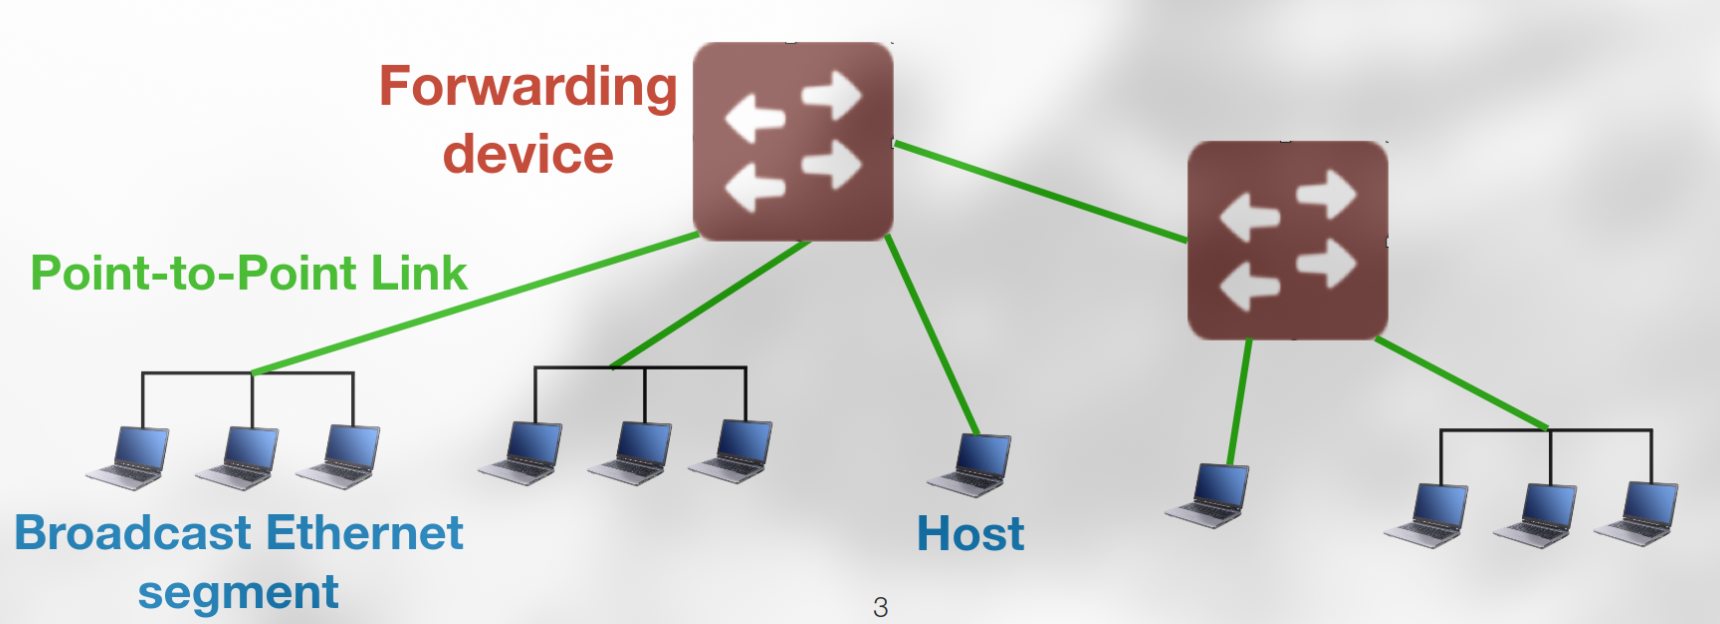
\includegraphics{images/forwarding-device.png}
    \caption{Forwarding Device}
    \label{fig:forwardingdevice}
\end{figure}
A point-to-point forwarding device
typically comprises multiple ports (or network interfaces).
Each port connects to a single host or multiple hosts sharing a
medium or some other forwarding device, using point-to-point links.
It forwards packets received on one port out on some other port.

There are three layers for forwarding devices, although a given
device can function at multiple layers:
\begin{itemize}
    \item Layer 1: operates at Physical layer, i.e.,
          forwards using physical layer
          packet header fields. Example: a Hub
    \item Layer 2: operates at Data Link layer, i.e.,
          forwards using Data Link layer
          packet header fields (e.g., using destination MAC address).
          Example: a bridge or switch.
    \item operates at Network layer, i.e., forwards using Network layer
          packet header fields (e.g., using destination IP address).
          Example: a router.
\end{itemize}

\paragraph{Layer 1} A layer 1 device, the hub, is the simplest possible
forwarding device. It broadcasts frame received on a given port to all
other ports except the port the frame was received on.
Physical layer headers contain no address information, so broadcast is
the only option. Typically a hub connects multiple Broadcast Ethernet segments.
and helps extend Broadcast Ethernet to larger distance
by providing signal amplification and signal re-generation. Nobody really uses
hubs these days because they just create bigger Ethernet segments,
which still have collisions.

\paragraph{Layer 2} The simplest layer 2 device is a bridge. It understands
MAC addresses and creates two half-duplex point-to-point connections
between its two ports. A generalized version of the bridge, the switch,
is the most commonly used device. A switch is a multi-port bridge, i.e.,
has $N > 2$ ports. It creates $N$ half-duplex point-to-point connections
(a \emph{matching}) between input and output ports using a crossbar,
which is just a bunch of wires going between input and output ports.
A matching is a bipartite graph
where every edge has a unique endpoint.

An algorithm
called iSLIP decides the matching configuration.
iSLIP looks at the current \emph{demand}, i.e., for each input packet
what is the output port.
iSLIP then configures the crossbar to create the matching that satisfies
the most demands.
It repeats the above two steps iteratively till all demands are satisfied.

Ethernet running inside a switch is called “Switched Ethernet”.
Modern Ethernet LANs run Switched Ethernet
instead of Broadcast Ethernet.

In switched ethernet, each switch maintains a “Forwarding Table”
Which keeps track of which hosts are reachable via each output port.
For the network in Figure \ref{fig:switchedethernetnetwork}, the
forwarding table is given by the table below.
\begin{figure}
    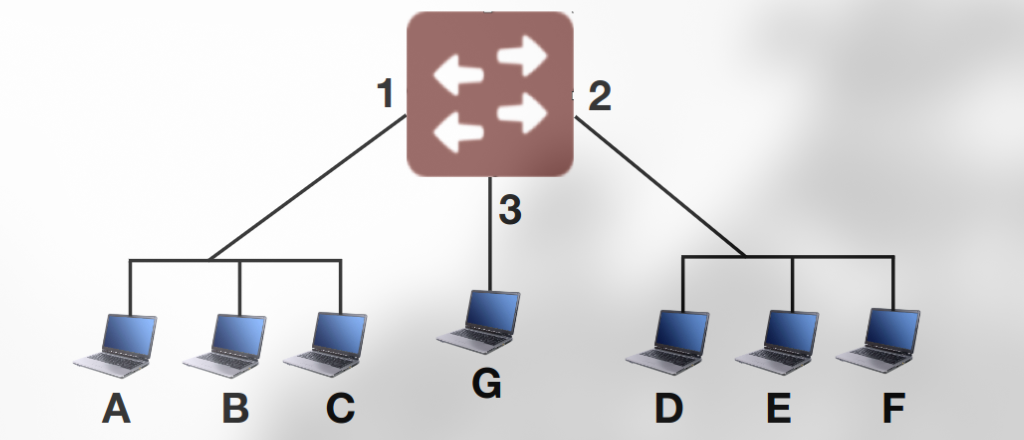
\includegraphics{images/switchedethernetnetwork.png}
    \caption{Switched Ethernet Network}
    \label{fig:switchedethernetnetwork}
\end{figure}

\begin{table}[h]
    \centering
    \begin{tabular}{|c|c|}
        \hline
        \textbf{Destination MAC Address} & \textbf{Output Port} \\ \hline
        A.mac                            & 1                    \\ \hline
        B.mac                            & 1                    \\ \hline
        C.mac                            & 1                    \\ \hline
        D.mac                            & 2                    \\ \hline
        E.mac                            & 2                    \\ \hline
        F.mac                            & 2                    \\ \hline
        G.mac                            & 3                    \\ \hline
    \end{tabular}
\end{table}

To populate the forwarding table, use the following algorithm.
When a switch receives a frame on port p, it checks the source
MAC address in the frame. Let it be $s$.
The switch learns that host with MAC address $s$ is reachable via port $p$,
so it adds the entry $<s, p>$ to its forwarding table.
If a switch never receives a frame sourced from a host, it
will never learn which port the host is reachable on.

The way MAC forwarding works is that, upon receiving a frame with destination
MAC $d$ and if \texttt{d = ff:ff:ff:ff:ff:ff}, copy and send frame on every
port except the port on which the frame was received on. This is a broadcast.
If $d$ is not \texttt{ff:ff:ff:ff:ff:ff}, then check the forwarding table
for an entry $<d, p>$. If entry $<d, p>$ exists, then if $p$ is same as the
port on which frame was received, then drop the frame. Otherwise send frame
out on port $p$. Else if no entry corresponding to $d$ exists, the switch
copies and sends frame on every port except the port on
which the frame was received on, again a broadcast. If there is a loop
in the network graph, then a broadcast packet can cause infinite loops
and consume all resources in a broadcast storm. The way to avoid this
is to structure networks as spanning trees with no loops. Doing this
in a distributed way is extremely complex.

\subsection{Network}

\subsection{Transport}

\subsection{Application}


